\documentclass{beamer}

\usepackage[utf8]{inputenc}
\usepackage[T1]{fontenc}
\usepackage{amsmath}
\usepackage{bm}

\usepackage{tabularx}
\usepackage{graphicx}
\usepackage{epstopdf}
\usepackage{multirow}
\usepackage{natbib}

\graphicspath{{../../images/}}

\usetheme{Madrid}
\usebeamercolor{sidebartab}
\usefonttheme{professionalfonts}

\setbeamertemplate{caption}{\raggedright\insertcaption\par}


\title[M.Sc. Thesis 2015]{Probabilistic Modeling of City-scale Image Collections}
\author{Diego A. Ballesteros Villamizar}
\institute[ETHZ]{ETH Zürich}
\date{April 26th, 2016}

\DeclareMathOperator*{\argmin}{argmin}
\DeclareMathOperator*{\argmax}{argmax}

\AtBeginSection[]
{
  \begin{frame}<beamer>
    \frametitle{Outline}
    \tableofcontents[currentsection]
  \end{frame}
}

\begin{document}

\begin{frame}
  \titlepage
\end{frame}

\section{Introduction}

\begin{frame}{Touristic Route Planning}
  Let's plan a 2-day trip to Zürich. How can we go from this?
  \begin{figure}
    \centering
    \includegraphics[scale=0.3]{tripadvisor}
  \end{figure}
\end{frame}

\begin{frame}{Touristic Route Planning}
  To this:
  \begin{figure}
    \centering
    \includegraphics[scale=0.2]{routes_1}
  \end{figure}
\end{frame}

\begin{frame}{Related Work: Mapping the World's Photos}
  \begin{itemize}
    \item "Photo shots are a prime element of the image perceived by visitors and also a path to understanding processes in the symbolic construction of destinations." \citet{Donaire2014}
    \item \citet{Kleinberg2009} used mean-shift clustering to identify highly photographed locations.
  \end{itemize}
  \begin{figure}\centering
    \includegraphics[scale=0.15]{kleinberg2009}
    \caption{Representative photos for top landmarks in North America identified from Flickr data. Source: \citet{Kleinberg2009}}
  \end{figure}
\end{frame}

\begin{frame}{Related Work: Travel Route Recommendation Using Geotags in Photo Sharing Sites}
  \begin{itemize}
    \item \citet{Kurashima2010} modeled photographer behavior by combining Markov and topic models in a probabilistic framework.
  \end{itemize}
  \begin{columns}
    \begin{column}{0.3\textwidth}
      \begin{figure}
        \centering
        \includegraphics[width=\textwidth]{kurashima1}
        \caption{Highly photographed locations. Source: \citet{Kurashima2010}}
      \end{figure}
    \end{column}
    \pause
    \begin{column}{0.3\textwidth}
      \begin{align*}
        P(l_{t} \mid l_{t-1}, h^{u}) \\
        P(l_{t} \mid l_{t-1}) \\
        \sum_{z \in \bm{Z}}P(z \mid h^{u})P(l_{t} \mid z) \\
      \end{align*}
      Markov and Topic models.
    \end{column}
    \pause
    \begin{column}{0.3\textwidth}
      \begin{figure}
        \centering
        \includegraphics[width=\textwidth]{kurashima2}
        \caption{Routes from the model. Source: \citet{Kurashima2010}}
      \end{figure}
    \end{column}
  \end{columns}
\end{frame}

\begin{frame}{Sets of Locations to Visit}
  \begin{itemize}
    \item Let's simplify the problem and focus on which locations to visit.
    \item The when and how can be determined later.
    \item Instead of:
  \end{itemize}
  \begin{figure}
    \centering
    \includegraphics[scale=0.15]{routes_1}
  \end{figure}
\end{frame}

\begin{frame}{Sets of Locations to Visit}
  \begin{itemize}
    \item Let's simplify the problem and focus on which locations to visit.
    \item The when and how can be determined later.
    \item We aim to identify:
  \end{itemize}
  \begin{figure}
    \centering
    \includegraphics[scale=0.3]{sets_1}
  \end{figure}
\end{frame}

\begin{frame}{Good Sets of Locations}
  Let's try to build one, first a highly popular location: Grossmünster
  \begin{columns}
    \begin{column}{0.5\textwidth}
      \begin{figure}
        \centering
        \includegraphics[width=\textwidth]{diversity_set_1}
      \end{figure}
    \end{column}
    \begin{column}{0.5\textwidth}
      \begin{figure}
        \centering
        \includegraphics[width=.5\textwidth]{grossmunster}
        \caption{Grossmünster. Source: \url{https://commons.wikimedia.org/w/index.php?curid=5082760}}
      \end{figure}
    \end{column}
  \end{columns}
\end{frame}

\begin{frame}{Diverse Sets of Locations}
  The next on the list of top attractions is Fraumünster, but two churches on the same day? Let's add a museum instead.
  
  \begin{columns}
    \begin{column}{0.5\textwidth}
      \begin{figure}
        \centering
        \includegraphics[width=\textwidth]{diversity_set_2}
      \end{figure}
    \end{column}
    \begin{column}{0.5\textwidth}
      \begin{figure}
        \centering
        \includegraphics[width=.7\textwidth]{landesmuseum}
        \caption{Swiss National Museum. Source: \url{https://commons.wikimedia.org/w/index.php?curid=7974880}}
      \end{figure}
    \end{column}
  \end{columns}
\end{frame}

\begin{frame}{Diverse Sets of Locations}
  And so on...
  \begin{figure}
    \centering
    \includegraphics[width=.55\textwidth]{diversity_set_3}
  \end{figure}
\end{frame}

\begin{frame}{Complementary Sets of Locations}
  \begin{itemize}
    \item Only diversity? What about tourists interested in a coherent theme?
    \item Perhaps a trip through stores in Zürich.
  \end{itemize}
  \begin{figure}
    \centering
    \includegraphics[width=.5\textwidth]{coherent_set}
  \end{figure}
\end{frame}

\begin{frame}{Choosing a Model}
  \begin{itemize}
    \item Modeling sets of items $\rightarrow$ Functions over sets
    \item Diversity $\rightarrow$ Submodularity
    \item Complementarity $\rightarrow$ Supermodularity
    \item Probabilistic modeling of tourist behavior $\rightarrow$ Probability of visiting a set of locations.
  \end{itemize}
\end{frame}

\begin{frame}{Diversity and Submodularity}
  \begin{itemize}
    \item Suppose a function $F(S)$ that sums the number of unique location types in $S$.
    \item For example, $F(\{$ETH, UZH$\}) = 1$, $F(\{$ETH, UZH, Fraumünster$\}) = 2$.
    \pause
    \item This is a submodular function.
    \pause
    \item Maximizing $F(S)$ for $S$ of fixed size implies adding locations of different types $\rightarrow$ Diversity.
  \end{itemize}
\end{frame}

\begin{frame}{Complementarity and Supermodularity}
  \begin{itemize}
    \item Suppose a function $F(S)$ that counts 1 for each pair of repeated location types in $S$.
    \item For example, $F(\{$ETH, UZH, Fraumünster$\}) = 1$, $F(\{$ETH, Fraumünster$\}) = 0$.
    \pause
    \item This is a supermodular function. 
    \pause
    \item Maximizing $F(S)$ for $S$ of fixed size implies adding locations of the same types $\rightarrow$ Complementarity.
  \end{itemize}
\end{frame}

\begin{frame}{Probabilistic Submodular Models}
  \begin{itemize}
    \item Probabilistic Submodular Models (PSMs) are a class of distributions over the powerset of a set $V$ of the form
      \begin{equation*}
      P(S) = \frac{\exp{F(S)}}{Z}
      \end{equation*}
     for all $S \subset V$,  where F(S) is submodular or supermodular. These distributions are log-submodular and log-supermodular, respectively.
   
     \item Inference in these distributions has been recently studied by \cite{djolonga15scalable} and \cite{gotovos15sampling}.
  \end{itemize}
\end{frame}

\begin{frame}{Learning PSMs}
  \begin{itemize}
    \item We are interested in applying these distributions to a dataset of geotagged photographs. \citet{tschiatschek16learning} studied learning a PSM from data, i.e. estimating the model parameters.
    \item Maximum Likelihood Estimation is not tractable, because the exact computation of the partition function $Z$ is \#P-complete.
    \item Noise Contrastive Estimation (NCE) was used as an alternative for learning the PSM.
    \item We'll take a closer look at the model proposed by \citet{tschiatschek16learning}.
  \end{itemize}
\end{frame}

\begin{frame}{Noise Contrastive Estimation}
  \begin{itemize}
    \item Transform the task of estimating a distribution into a supervised learning task, namely a classification task.
    \item Noise samples $\mathcal{N}$ are drawn from a known normalized distribution $P_{n}$ and contrasted with the data samples $\mathcal{D}$ assumed to come from a distribution $P_{d}$.
    \item Partition function $Z$ becomes one of the parameters to estimate.
    \item Stochastic Gradient Descent can be used to optimize the classification objective.
  \end{itemize}
\end{frame}

\section{Facility Location Diversity}

\begin{frame}{Submodular Model for Diversity}
  \begin{itemize}
    \item A submodular function for diversity,
      \begin{equation*}
        F(S) = u(S) + D(S)
      \end{equation*}
    where $u(S)$ aggregates the utility of the items in $S$ and $D(S)$ quantifies the diversity of the items in $S$.
   \item The corresponding PSM is:
     \begin{equation*}
       P(S) = \frac{1}{Z}\exp{\left(u(S) + D(S)\right)}
     \end{equation*}
   \item This is the general form of the Facility Location Diversity (FLID) model proposed by \citet{tschiatschek16learning}.
  \end{itemize}
\end{frame}

\begin{frame}{Aggregating Utility}
  \begin{itemize}
    \item A (sub)modular function
      \begin{equation*}
        u(S) = \sum_{i \in S}u_{i}
      \end{equation*}
    where $u_{i}$ represents the utility of each item $i$ in the ground set $V$.
    \item For example, the utility of a location could be the number of users that have taken photos of it.
  \end{itemize}
\end{frame}

\begin{frame}{Quantifying Diversity (Simplified)}
  \begin{itemize}
    \item A submodular function
      \begin{equation*}
        D_{d}(S) = \max_{i \in S}w_{i,d} - \sum_{i \in S}w_{i,d}
      \end{equation*}
    where $w_{i}$ quantifies the contribution of item $i$ to some concept $d$ related to the diversity of the set.
    \item For example, for the concept "is a museum" locations may have binary weights $w_{d} \in \{0,1\}$. Then a set with many museums is penalized with a negative value of $D_{d}(S)$
  \end{itemize}
\end{frame}

\begin{frame}{Quantifying Diversity}
  \begin{itemize}
    \item FLID uses $L$ dimensions capturing some diversity concepts. Each item can be represented with a vector $\mathbf{w}_{i} \in \mathbb{R}^{L}_{\geq 0}$.
  \end{itemize}
  \begin{columns}
    \begin{column}{0.45\textwidth}
      \begin{figure}
        \centering
        \includegraphics[width=\textwidth]{fldc_toy_example_diversity_weights}
      \end{figure}
    \end{column}
    \begin{column}{0.45\textwidth}
      \begin{figure}
        \centering
        \includegraphics[width=\textwidth]{disjoint_pairs}
      \end{figure}
    \end{column}
  \end{columns}
  
\end{frame}

\begin{frame}{FLID}
  \begin{equation*}
    P(S) = \frac{1}{Z}\exp{\left(\sum_{i \in s} u_{i} + \sum_{d=1}^{L}\max_{i \in S}{w_{i,d} - \sum_{i \in S}w_{i,d}}\right)}
  \end{equation*}
  \begin{itemize}
    \item Learning can be performed efficiently, in $\mathcal{O}(|\mathcal{D} \cup \mathcal{N}|L\kappa)$ where $\kappa = \argmax_{S \in \mathcal{D} \cup \mathcal{N}}|S|$.
    \item For small $L$, exact computation of $Z$ is feasible.
    \item Applications shown by \citet{tschiatschek16learning}:
      \begin{itemize}
        \item Product recommendation with Amazon baby registries.
        \item Summarization of an image collection.
      \end{itemize}
  \end{itemize}
\end{frame}

\section{Beyond Diversity: FLDC}

\begin{frame}{Quantifiying Complementarity}
  \begin{figure}
    \centering
    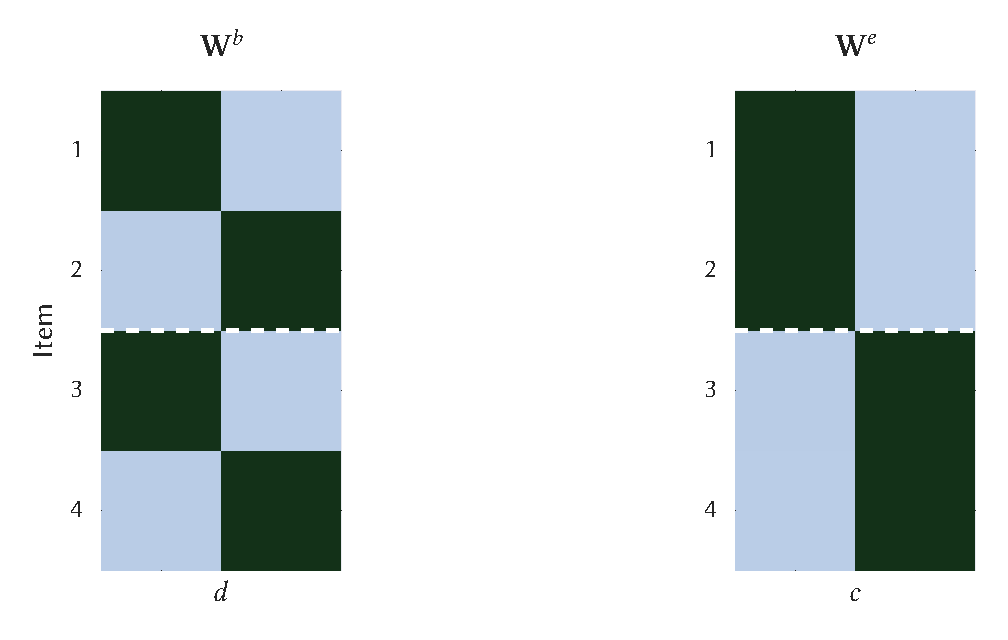
\includegraphics[height=.8\textheight]{fldc_toy_example_mixed_weights_pres}
  \end{figure}
\end{frame}

\begin{frame}{Facility Location Diversity and Coherence}
  \begin{itemize}
    \item We propose adding a similar supermodular term to FLID to model complementarity.
      \begin{equation*}
        P(S) = \frac{1}{Z}\exp{\left(u(S) + D(S) + \sum_{c=1}^{K}\sum_{i \in S}w^{e}_{i,c} - \max_{i \in S}{w^{e}_{i,c}}\right)}
      \end{equation*}
   \item Complexity of learning is only increased by a factor of $K$.
  \end{itemize}
\end{frame}

\begin{frame}{Experimental Setup: Data and Clustering}
  \begin{columns}
    \begin{column}{0.45\textwidth}
      \begin{figure}
        \centering
        \includegraphics[width=\textwidth]{zurich_feature_map_2015}
        \caption{Geotagged photos from Flickr.}
      \end{figure}
    \end{column}
    \begin{column}{0.45\textwidth}
      \begin{figure}
        \centering
        \includegraphics[width=\textwidth]{top_100_zurich}
        \caption{Top photographed locations.}
      \end{figure}
    \end{column}
  \end{columns}
\end{frame}

\begin{frame}{Experimental Setup: Completing Sets}
  \begin{itemize}
    \item Geotagged photos were grouped by user and day they were taken.
    \item Each group represents a set. Test sets are constructed by taking out one element at a time.
    \item For example, if the original set is \textit{\{Fraumünster, Grossmünster, Hauptbahnhof\}}, the test sets are:
      \begin{itemize}
        \item \textit{\{Fraumünster, Hauptbahnhof\}}
        \item \textit{\{Grossmünster, Hauptbahnhof\}}
        \item \textit{\{Fraumünster, Grossmünster\}}
      \end{itemize}
  \end{itemize}
\end{frame}

\begin{frame}{Experimental Setup: Baselines}
  \begin{itemize}
    \item The test set is $S = \{l_{1}, \dots, l_{n}\} \setminus \{l_{t}\}$.
    \item Modular
      \begin{equation*}
         \argmax_{i \notin S} u_{i}
      \end{equation*}
    \item Proximity
      \begin{equation*}
        \argmin_{i \notin S} \sum_{j \in S}d(i,j)
      \end{equation*}
    \item FLID
      \begin{equation*}
        \argmax_{i \notin S} P_{FLID}(S)
      \end{equation*}
  \end{itemize}
\end{frame}

\begin{frame}{Experimental Setup: Ordered Baselines}
  \begin{itemize}
    \item The ordered test set is $S_{n} = [l_{1}, \dots, l_{t-1}, l_{t+1}, \dots, l_{n}]$.
    \item Markov model
      \begin{equation*}
        \argmax_{i \in V} P(i \mid l_{t-1})P(l_{t+1} \mid i)
      \end{equation*}
    \item Heuristic Markov model
      \begin{equation*}
        \argmax_{i \notin S_{n}} P(i \mid l_{t-1})P(l_{t+1} \mid i)
      \end{equation*}
    \item Proximity ordered model
      \begin{equation}
        \argmin_{i \notin S_{n}} d(i, l_{t-1}) + d(i, l_{t+1})
      \end{equation}
  \end{itemize}
\end{frame}

\begin{frame}{Results - Accuracy}
  \begin{figure}
    \centering
    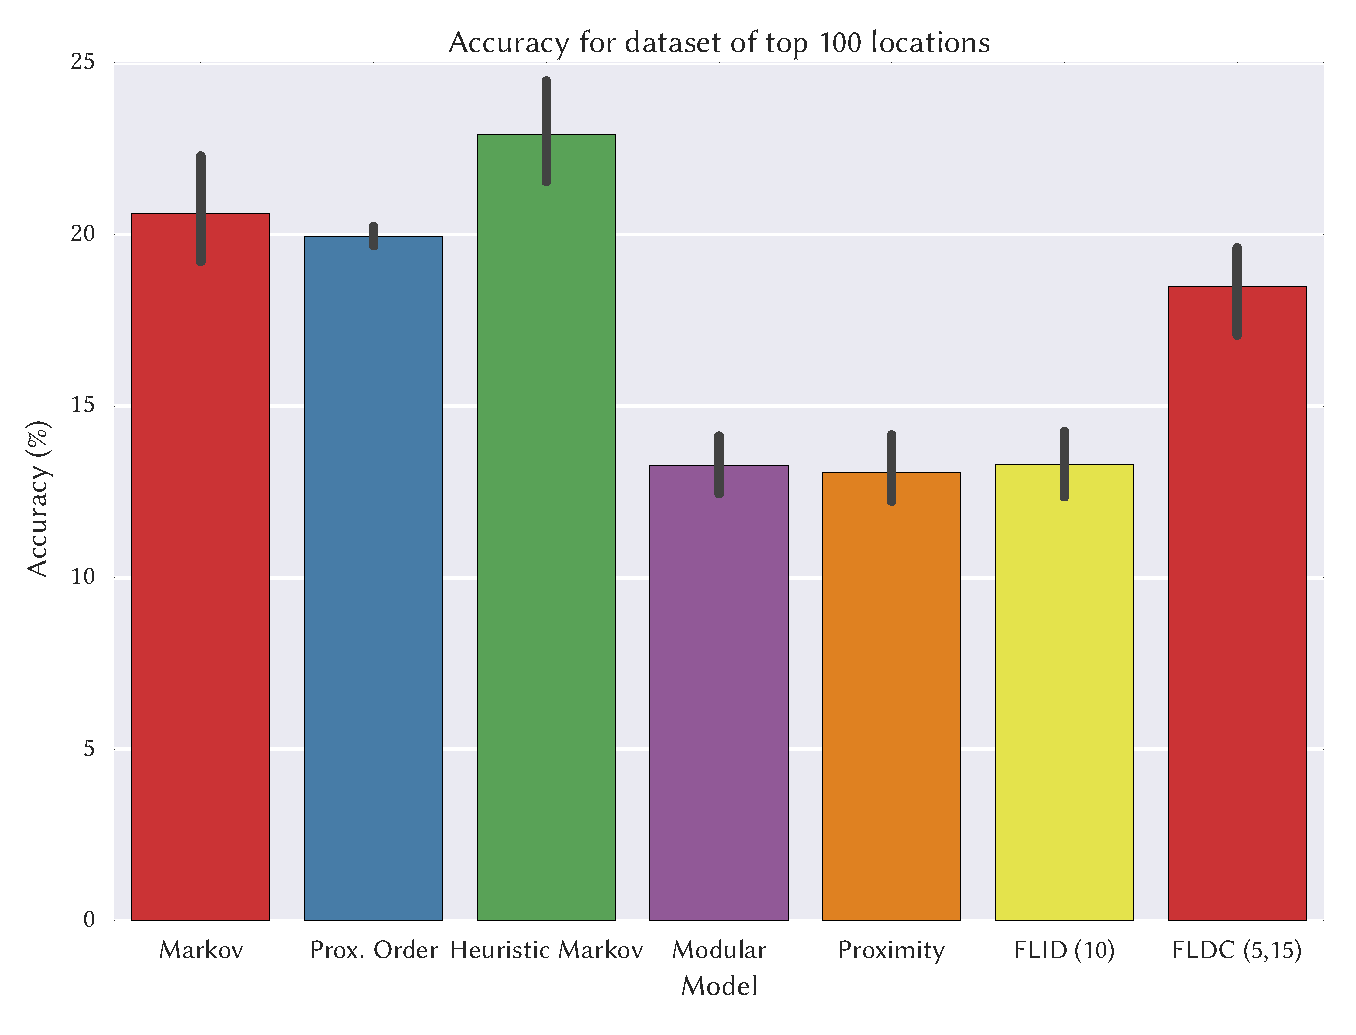
\includegraphics[width=.85\textwidth]{all_models_100_presentation}
  \end{figure}
\end{frame}

\section{Generalizing: FFLDC}

\begin{frame}{How to Generalize?}
  \begin{itemize}
    \item Is it possible to transfer knowledge about Zürich to Geneva?
    \item If new locations are identified, how can they be included in the model without learning it again?
    \item Our proposed solution: \textbf{Featurized representations}.
  \end{itemize}
\end{frame}

\begin{frame}{Featurized Facility Location Diversity and Coherence}
  \begin{itemize}
    \item Define a feature matrix for all items in $V$, i.e. $\mathbf{X} \in \mathbb{R}^{|V| \times M}$.
    \item Factorize the model parameters $\mathbf{u}, \mathbf{W}^{b}, \mathbf{W}^{e}$
      \begin{align*}
        \mathbf{u} &= \mathbf{X}\mathbf{a} \\
        \mathbf{W^{b}} &= \mathbf{X}\mathbf{B} \\
        \mathbf{W^{e}} &= \mathbf{X}\mathbf{E}
      \end{align*}
    \item Model is then defined in the space of features, not items.
  \end{itemize}
\end{frame}

\begin{frame}{Experimental Setup: Locations}
  A smaller dataset with 10 locations.
  \begin{itemize}
    \item Hauptbahnhof
    \item Fraumünster
    \item Grossmünster
    \item Hallenstadion
    \item Prime tower
    \item Bürkliplatz
    \item Paradeplatz
    \item Bellevueplatz
    \item Rathaus
    \item Zoo
  \end{itemize}
\end{frame}

\begin{frame}{Experimental Setup: Features}
  \begin{itemize}
    \item Is it a transit station? E.g. Hauptbahnhof, Bürkliplatz.
    \item Is it a church? E.g. Fraumünster.
    \item Is it a historic building? E.g. Grossmünster, Rathaus.
    \item Is it an indoors location? E.g. Prime tower, Hallenstadion.
    \item Normalized number of photographs $n_{p}$, $\sqrt{n_{p}}$ and $\sqrt[4]{n_{p}}$.
    \item Number of users per photograph.
  \end{itemize}
\end{frame}

\begin{frame}{Experimental Setup: Evaluation}
  \begin{equation*}
    \mathrm{LLRI} = 100\frac{\mathcal{L}_{model} - \mathcal{L}_{log-modular}}{|\mathcal{L}_{log-modular}|}
  \end{equation*}
  \begin{itemize}
    \item It measures the model fit on test data.
    \item For the small dataset, the accuracy is already at 40\% with the modular model and does not improve.
  \end{itemize}
\end{frame}

\begin{frame}{Results - LLRI}
  \begin{figure}
    \centering
    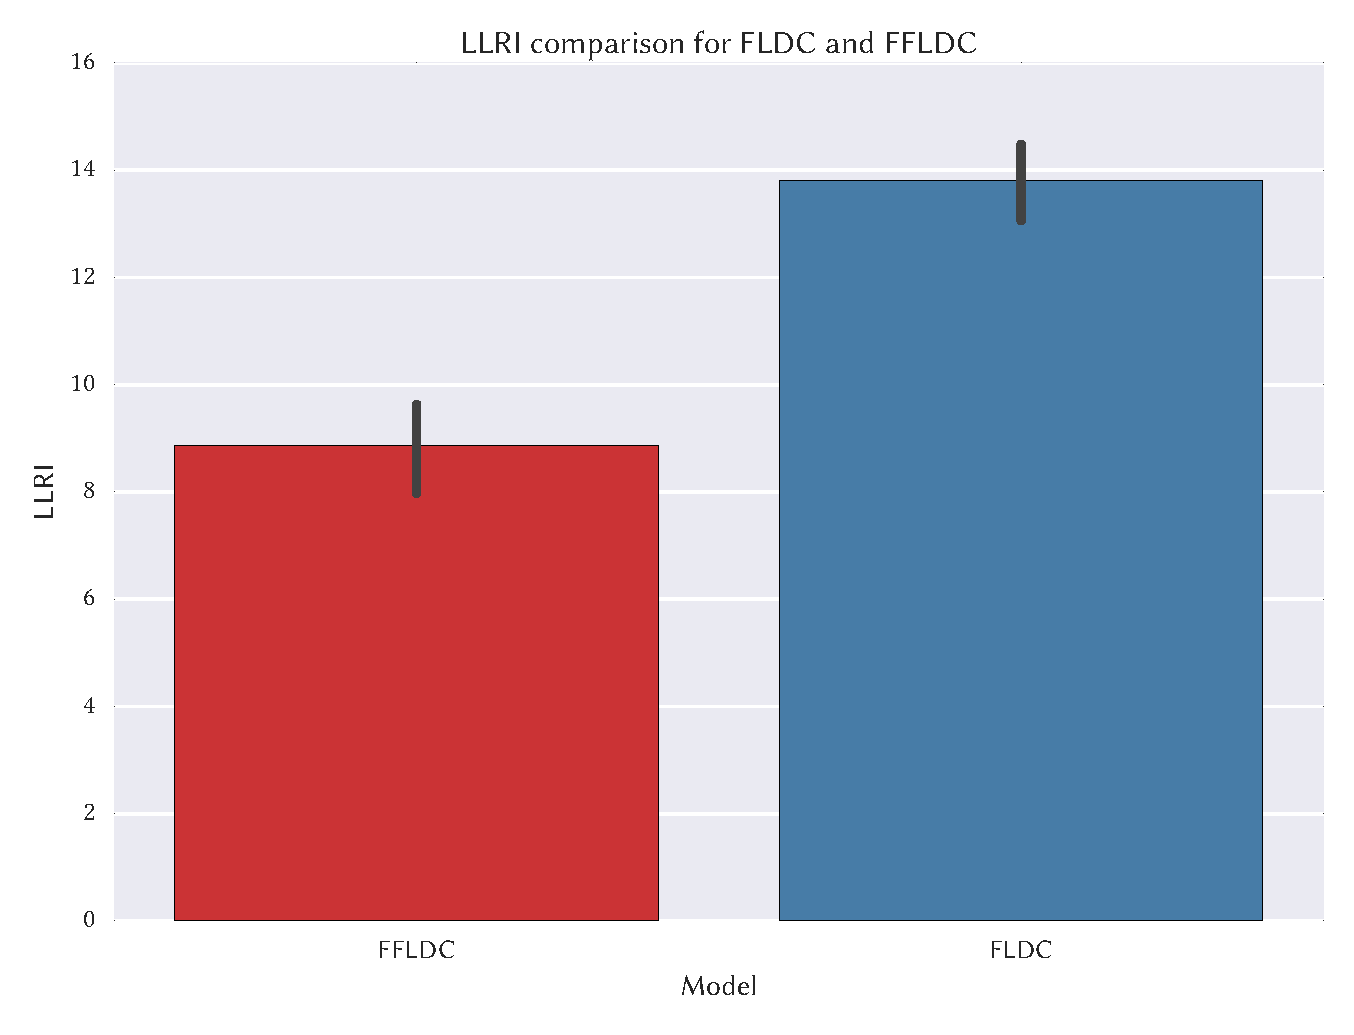
\includegraphics[width=.8\textwidth]{ffldc_10_llri}
  \end{figure}
\end{frame}

\section{Conclusion}

\begin{frame}{Conclusions}
 \begin{itemize}
   \item We have proposed an extension of FLID to model complementarity or attractiveness in sets.
   \item Experiments in a real world application show how this can improve the quality of the model.
   \item Recommendation of tourist locations can be modeled using PSMs with positive results. However, modeling of ordered sets is an important direction to explore.
   \item We have proposed an extension of FLID to generalize the model to unseen items through features.
  \end{itemize}
\end{frame}

\begin{frame}[allowframebreaks]{References}
  \bibliographystyle{apalike}
  \bibliography{../report/bibliography/references}
\end{frame}

\end{document}
